\chapter{XLore系统与应用接口构建}
\label{cha:xlore}

\section{本章引论}

跨语言知识库对全球知识的共享有着很大贡献。然而,中英文的跨语言知识库却很少,主要有以下几点原因:1)相对于丰富的英文知识,中文知识极度匮乏 2)现有中英文跨语言对应关系的缺乏。为解决以上问题,我们构建了一个大型中英文跨语言知识库(Cross-lingual Knowledge Base),该知识库命名为{\heiti XLore}。
%具体来说,XLore涵盖了英文维基,中文维基,百度百科与互动百科,四个在线百科的知识,以此来均衡中英文知识数量,同时,利用一个跨语言链接发现方法扩充跨语言链接集合,并引入了一个上下位关系判断,对分类树进行剪枝。详细流程见\ref{sec5:cross-lingual-knowledge-base}

当前一些知名的知识库会定期更新并发布自己的数据集,DBpedia\footnote{\url{http://wiki.dbpedia.org/}} 提供最新的数据集下载、数据统计记录,甚至开源代码;Probase\footnote{\url{http://probase.msra.cn/Dataset.aspx}}给出语义关系的数据集供研究人员使用,如is-a关系,同义词等。
然而中文知识库领域,搜狗、百度等商业化知识图谱仅供自家公司商用,并没有开放数据。Zhishi.me\footnote{\url{http://zhishi.me/}}作为第一个科研领域的中文知识库,早期提供实体查询接口与SPARQL查询接口,现数据与网站都久未更新。

跨语言知识库XLore,提供了数据展示页面、知识搜索、SPARQL查询、实例关系可视化、实体链接等多项功能,本章将具体阐述XLore网站系统的搭建(详见\ref{sec5:system-describe}节)与实体链接接口的构建(详见\ref{sec5:entity-linking-api}节)。

\section{大规模中英文跨语言知识库XLore的构建}
\label{sec5:cross-lingual-knowledge-base}

XLore知识库融合中英文维基百科、百度百科与互动百科的信息,大大增加了中文知识数量,并利用大量跨语言链接提高中英文的融合度。其构建流程如图\ref{fig:xlore-preprocess},包括以下步骤:
\begin{enumerate}
\item 从维基的数据存储文件,与百度、互动百科的网页信息中抽取出结构化语义信息,主要包括概念、属性与实例三类元素的获取;
\item 生成跨语言链接集合,包括维基百科跨语言链接、通过文献\cite{wang2012cross}中的方法计算出的扩展链接、以及\ref{sec:cross-lingual-seed}节中生成的属性跨语言链接;
\item 运用文献\cite{wang2014cross}中提出的语义关系验证方法,对上下文关系进行判断与剪枝;
\item 将数据转换成RDF三元组格式,导入到Virtuoso数据库。
\end{enumerate}

\begin{figure}[ht]
  \centering
  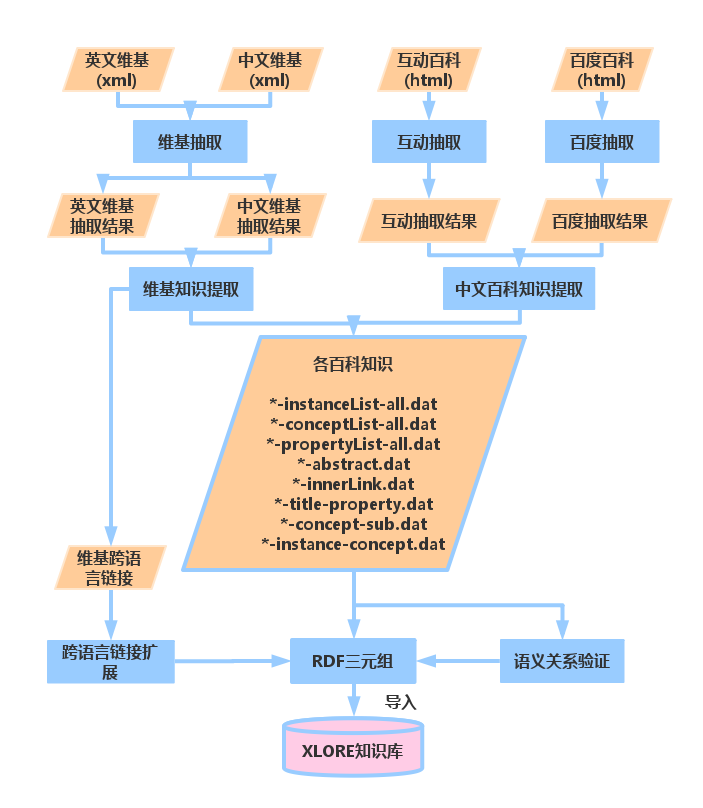
\includegraphics[width=0.8\columnwidth]{xlore_preprocess}
  \caption{跨语言知识库XLore构建流程}
  \label{fig:xlore-preprocess}
\end{figure}

最终数据转化成标准RDF,比如:以$\langle$\emph{http://xlore.org/instance/id}$\rangle$类型的URI 标识实例,使用\textit{owl:subClassOf}关系表征两个概念的关系。其中,跨语言的知识信息,如标签等,会通过@en与@zh区分,形成两类知识信息;跨百科知识信息,如摘要、源URL等,会通过@enwiki, @zhwiki, @baidu, @hudong区分成来源。

\subsection{抽取结果与统计}
本小节给出XLore知识库的知识数量统计结果,其中表\ref{tab:extract-result}为从各百科中抽取的概念、属性、实例数量统计,表\ref{tab:xlore-result}为融合后最终知识库中知识数量。

\begin{table}[htb]
    \centering
  \begin{minipage}[t]{0.8\linewidth}
    \caption{各元素抽取结果统计}
    \label{tab:extract-result}
    \begin{tabularx}{\linewidth}{lXXXX}
        \toprule[1.5pt]
               & 英文维基    & 中文维基   & 互动百科    & 百度百科     \\ \midrule[1pt]
        \#概念 & 982,432   & 159,705  & 31,802    & 1300      \\
        \#实例 & 4,304,113 & 662,650  & 5,590,751 & 5,622,404 \\
        \#属性 & 43,976    & 18,842   & 1187      & 139,634   \\
        \bottomrule[1.5pt]
    \end{tabularx}
  \end{minipage}
\end{table}

\begin{table}[htb]
    \centering
  \begin{minipage}[t]{0.9\linewidth}
    \caption{XLore结果展示}
    \label{tab:xlore-result}
    \begin{tabularx}{\linewidth}{lXXXXXX}
        \toprule[1.5pt]
        \multicolumn{1}{c}{} & \multicolumn{2}{c}{概念}     & \multicolumn{2}{c}{实例}                   & \multicolumn{2}{c}{属性}    \\ \midrule[1pt]
英文            & 639,020 & 96.26\%          & 3,879,121   & 38.79\%                & 15,380  & 27.24\%                \\
中文            & 88,615  & 13.35\%          & 7,409,519   & 68.25\%                & 51,618  & 91.44\%                \\
跨语言          & 63,895  & 9.63\%           & 432,598     & 3.98\%                 & 10,549  & 18.69\%                \\
%English O       & 575,125 & 86.65\%                & 3,446,523           & 31.75\%                & 4,831   & 8.56\%    \\ \hline
%Chinese O       & 24,720  & 3.72\%                 & 6,976,921           & 64,27\%                & 41,069  & 72.75\%   \\ \hline
总数           & 663,740 & {-}               & 10,856,042  & {-}                    & 56,449  & {-} \\
      \bottomrule[1.5pt]
    \end{tabularx}
  \end{minipage}
\end{table}

\section{XLore系统介绍}
\label{sec5:system-describe}
XLore网站\footnote{\url{http://xlore.org}}旨在对外展示系统收集和整理的语义数据与关系,并通过关键词搜索、可视化展示和数据接口等形式向用户提供便利的知识服务。

\subsection{XLore系统构建}
图\ref{fig:xlore-architecture}为XLore系统架构图。

\begin{figure}[ht]
  \centering
  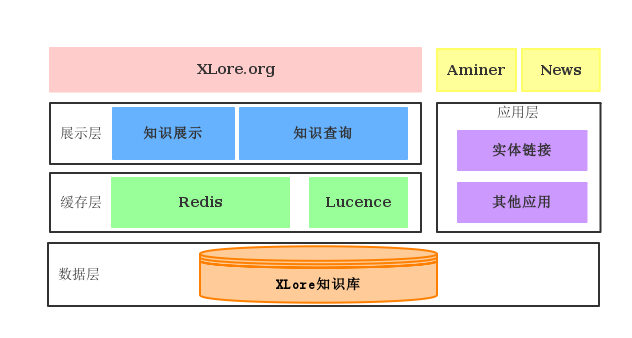
\includegraphics[width=0.9\columnwidth]{xlore-architecture}
  \caption{XLore系统架构图}
  \label{fig:xlore-architecture}
\end{figure}

为了语义化信息,我们将数据依托于图数据库。当前知名的的图数据库有Neo4J\footnote{\url{http://neo4j.com/}},AllegroGraph\footnote{\url{http://allegrograph.com/allegrograph/}},Virtuoso\footnote{\url{http://virtuoso.openlinksw.com/}}等,鉴于我们的数据是以三元组的形式组织的,更适用于triple—store类型的数据库,最终我们选用商业版Virtuoso(Virtuoso Universal Server)作为存储容器。

%Virtuoso是由OpenLink软件公司开发的一个混合型数据库,它既支持传统的RDBMS数据,也支持RDF等其他图类型数据的存储与查询。其商业版本(Virtuoso Universal Server)可支持多CPU处理、多会话访问以及集群网络环境等。商业版Virtuoso是闭源的,但OpenLink公司提供一个名为OpenLink Virtuoso的开源版本[GitHub链接],供使用者编译与尝试。

为了提高搜索效率,我们使用Redis\footnote{\url{http://redis.io/}}充当缓存。为了给出更好的搜索体验,用为各个元素标签及其URI建立了索引,使用Lucene的模糊查询代替完全匹配,返回更多相关搜索结果。

Web框架采用JSP+Struts2.0搭建,运行在Tomcat7.0 Web服务器上。

对于概念与实例,我们基于D3.js可视化库\footnote{\url{https://d3js.org/}},提供了关系可视化,包括概念-子概念的关系,实例-相关实例的关系。

\begin{figure}[ht]
  \centering
  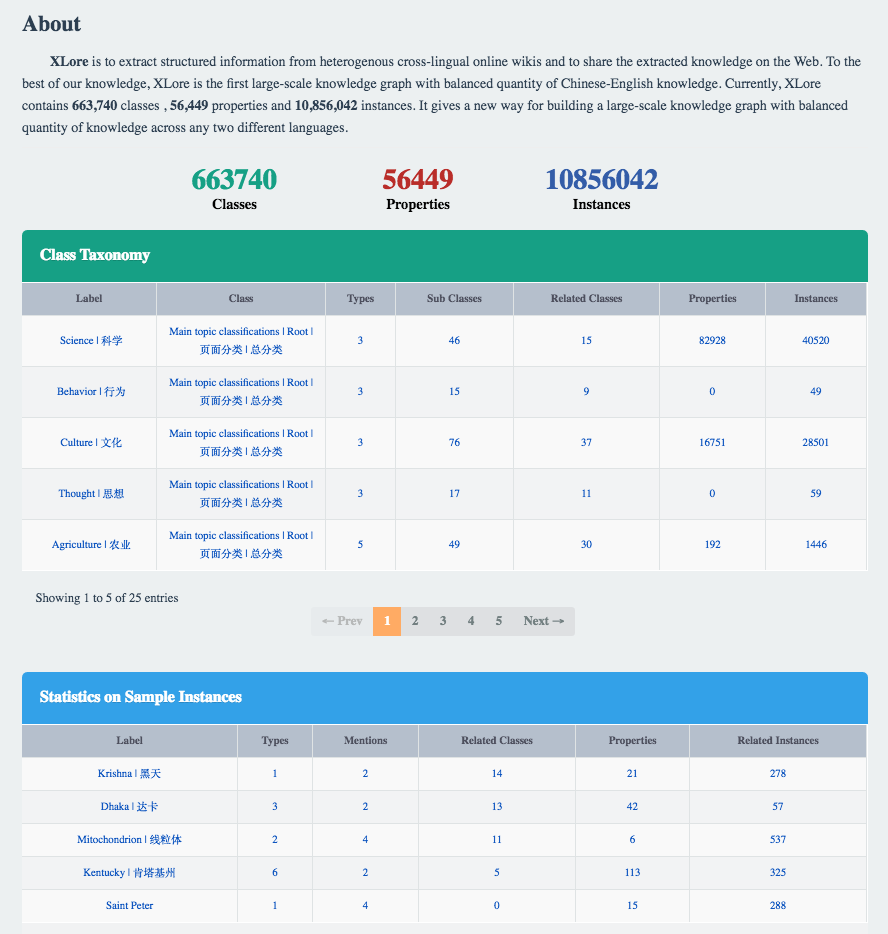
\includegraphics[width=0.8\columnwidth]{xlore-home}
  \caption{XLore网页系统首页}
  \label{fig:xlore-home}
\end{figure}

\subsection{XLore知识展示}
截止到2015年8月,XLore共收录663,740个概念、56,449个属性、10,856,042个实例。图\ref{fig:xlore-home}为XLore网站首页,以表格的形式提供了顶层及其下两层的概念层及其统计数据,列出的实例的样例数据,可直接点击查看相应实例页面。作为双语知识库,XLore提供了语言切换功能,同时满足中文与外文用户的语言需求。

XLore网站为三种知识提供展示,分别为概念、属性、实例。
概念页面以绿色为主色调,显示了概念中英文标签、父概念、子概念、相关实例等信息。
属性页面使用紫色色调,展示了中英文标签、属性类型(DateType与ObjectType)、相关实例、定义域(Domain)与值域(Range)等。
实例页面色调为蓝色,展示了中英文标签、实例图像、所属概念、摘要、信息框(包括中英文信息),URL 多种信息。三种页面中,涉及到的双语内容,我们以\textit{中文[英文]}的格式展示每条信息,如果用户的语言偏好设置为英文,则将英文展示在前,格式变为\textit{英文[中文]}。当涉及到四个百科内容且无法融合,我们利用网页标签分栏的形式分别展示不同百科信息,如图\ref{fig:xlore-page}。

\begin{figure}[ht]
  \centering
  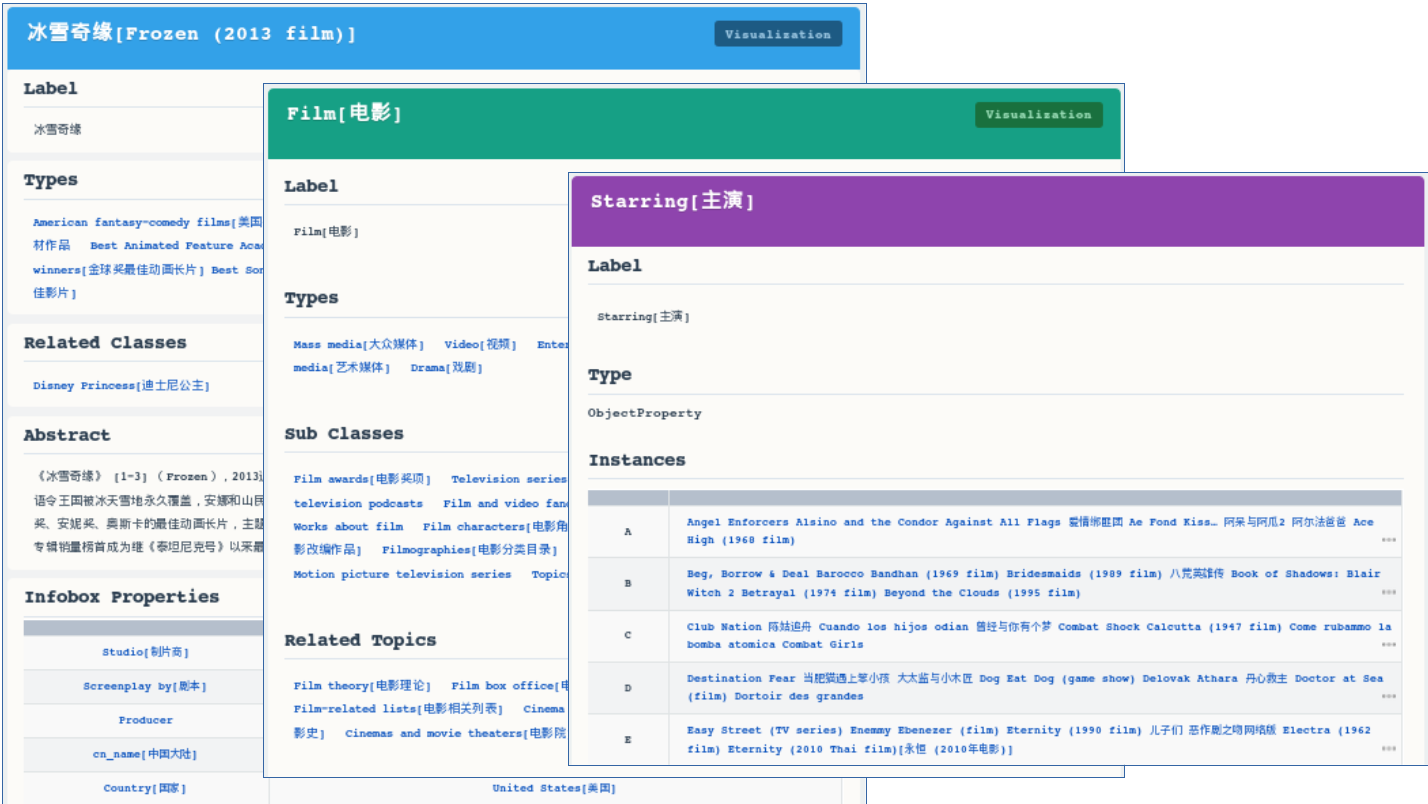
\includegraphics[width=1\columnwidth]{xlore-page}
  \caption{XLore实例、概念、属性页面展示}
  \label{fig:xlore-page}
\end{figure}

\subsection{XLore关系可视化}

XLore提供了两种数据可视化展示,分别为概念上下位关系可视化与相关实例可视化,图\ref{fig:xlore-visualization}分别给出了可视化样例,其中图\ref{fig:xlore-visualization-instance}显示指定实例及其相关实例,直接相关实例(信息框中实例)距离近,间接相关实例(文本内链接实例)距离较远,实例以领域划分,我们根据百科分类关系,定义14 个顶级概念,包括科学、社会、体育、经济等,实例被归属于距离最短的顶级概念中,如果距离多个概念一致,则通过投票机制决定,及选取到达次数最多的概念;图\ref{fig:xlore-visualization-concept}显示指定概念及其子概念(黄色)、父概念(绿色)。

\begin{figure}[ht]
  \centering
  \begin{subfigure}{7.2cm}
    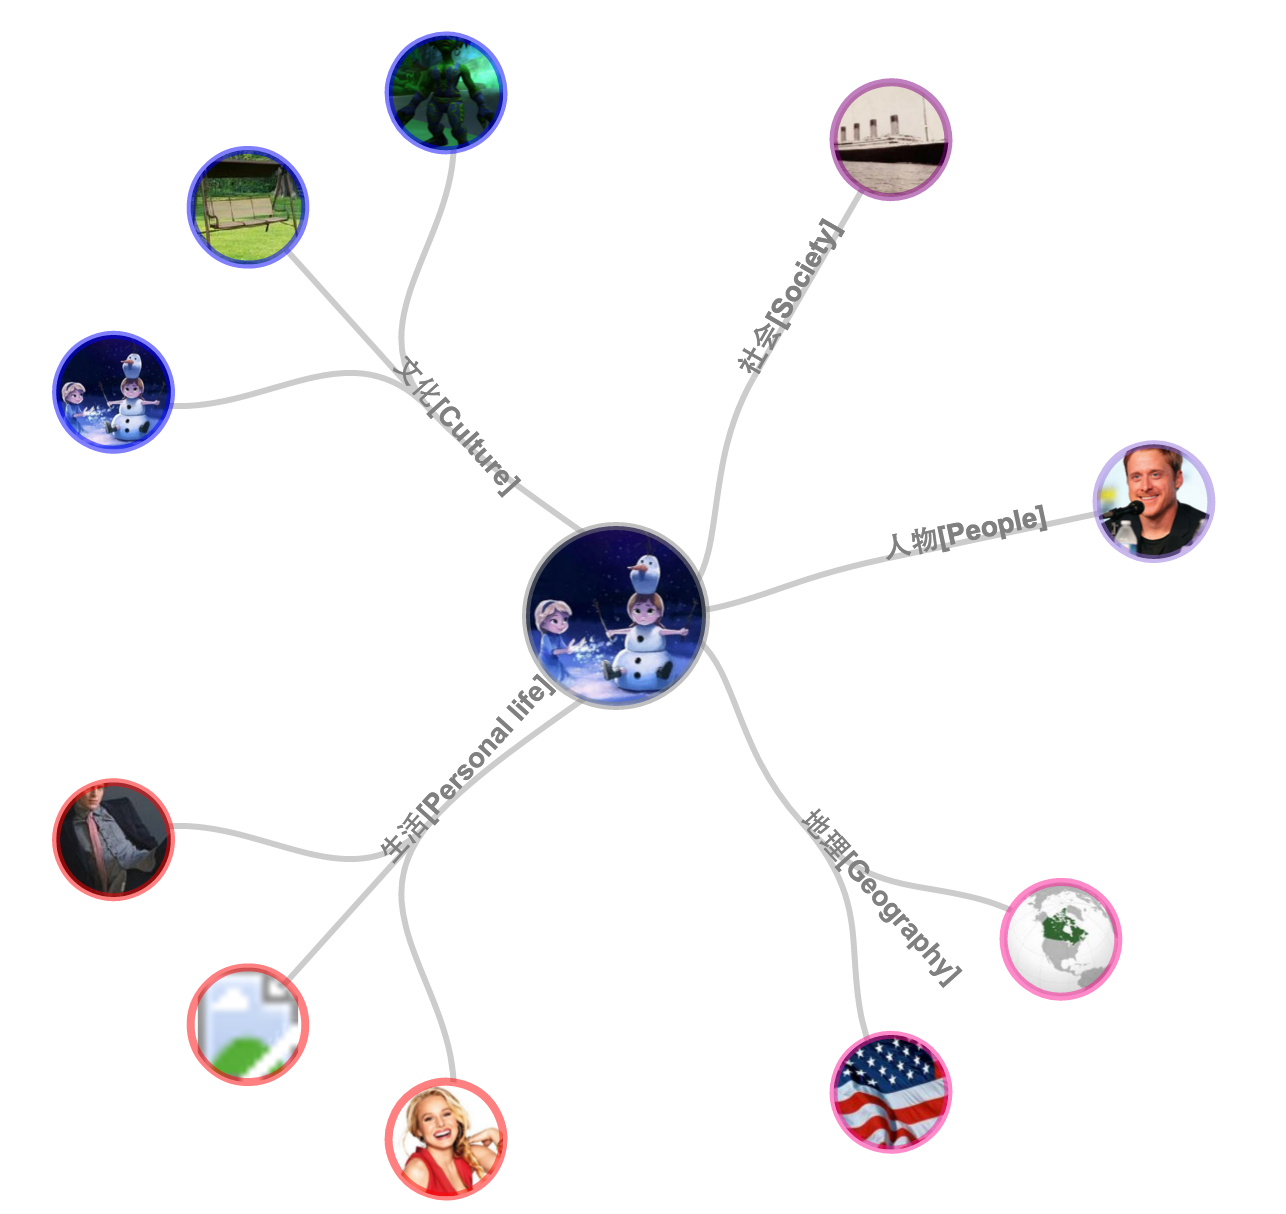
\includegraphics[height=5.4cm]{xlore-visualization-instance}
    \caption{实例可视化例子(阿甘正传)}
  \label{fig:xlore-visualization-instance}
  \end{subfigure}
  \hspace{0.01cm}%
  \begin{subfigure}{7.2cm}
    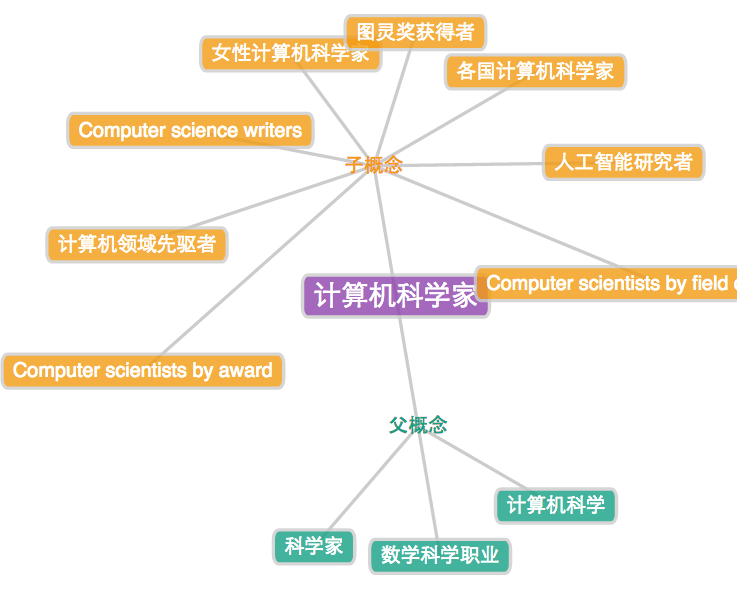
\includegraphics[height=5.4cm]{xlore-visualization-concept}
    \caption{概念可视化例子(计算机科学家)}
  \label{fig:xlore-visualization-concept}
  \end{subfigure}
  \caption{关系可视化例子}
  \label{fig:xlore-visualization}
\end{figure}

\subsection{XLore知识查询}
XLore提供搜索框文本查询与SPARQL语句查询两种查询方法。

搜索框显示于每个页面的上方,输入要查询的中文或英文字符串,即可获得模糊查询结果。默认情况下,系统会同时返回概念、属性和实例三类搜素结果,用户可根据具体的需求进行选择搜索。图\ref{fig:xlore-search-engine}为搜索结果页面展示。

\begin{figure}[ht]
  \centering
  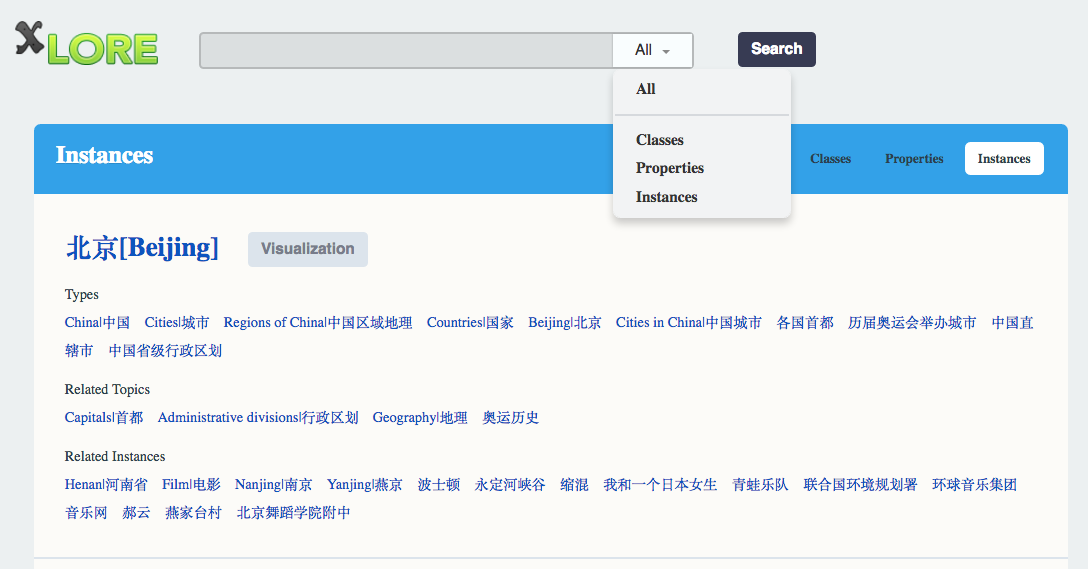
\includegraphics[width=0.9\columnwidth]{xlore-search-engine}
  \caption{XLore文本搜索框与搜索结果展示}
  \label{fig:xlore-search-engine}
\end{figure}

另一方面,对于专业人士,我们提供SPARQL查询页面。如图\ref{fig:xlore-sparql-endpoint}所示,输入正确的SPARQL语句,返回结果中可看到我们对知识库Schema的定义。另外,为了防止sql注入造成的攻击与数据库崩溃,我们添加了拦截器。

\begin{figure}[ht]
  \centering
  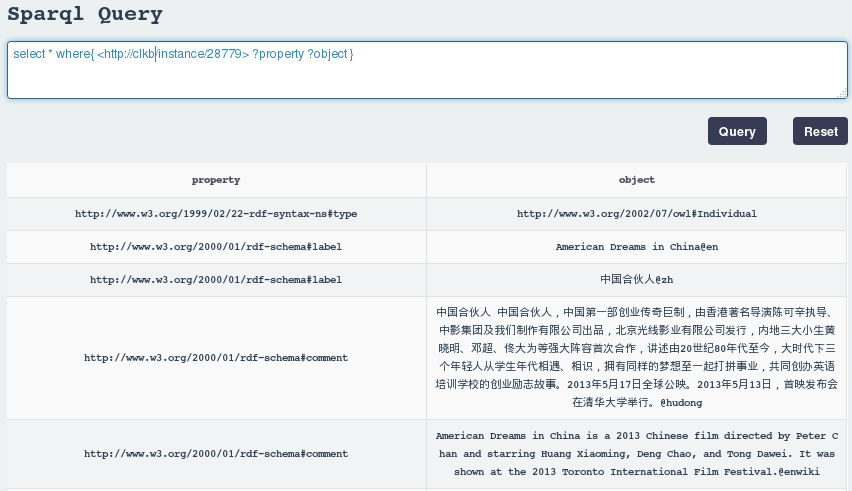
\includegraphics[width=0.9\columnwidth]{xlore-sparql-endpoint}
  \caption{XLore SPARQL 搜索框与搜索结果展示}
  \label{fig:xlore-sparql-endpoint}
\end{figure}

\section{XLore实体链接接口}
\label{sec5:entity-linking-api}

知识库的一个重要应用是实体链接(Entity Linking),
同一个实体可能有不同的称呼,比如演员刘德华,有昵称华仔、Andy。另一方面,一个名称可能表征不同实体,比如SVM在机器学习领域是\textit{Support Vector Machine}的缩写,但在新闻报道中可能是\textit{Stored Value Marketing公司}的简称。给出一个名称,在知识库中找出其对应的真正实体,被称作{\heiti 实体链接}任务。正确抽取出文本中的实体名称并准确链接到知识库中的对应实体,能够丰富文本中实体的上下文,对于文本的理解有很大意义。
实体链接是链接网络文本数据与知识库的桥梁,在很多不同领域中有所应用,比如信息抽取\cite{lin2012entity,nakashole2012patty}、文本分析\cite{gattani2013entity}、问答系统\cite{gattani2013entity}等等。TAC(Text Analysis Conference)将实体链接作为Knowledge Base Population(KBP)的一个子任务,并提供数据集供参赛者评测。

实体链接需要解决三个主要的子任务,即实体候选生成、实体候选排序、未链接文本预测。

{\heiti 实体候选生成}旨在建立一个名称与知识库实体的对应关系,实体链接的任务往往是首选在文本中识别出名称,再进一步分析可能对应的实体。因此实体候选是决定能否链接的关键步骤。通常情况下,实体候选集合从百科数据中抽取\cite{shen2012linden,shen2013linking},维基百科中的词条标题、重定向页面、消歧页面、超链接等,都可以作为实体名称。此外也有一些扩展方法,比如基于规则匹配\cite{han2009nlpr_kbp,lehmann2010lcc},取公司首字母缩写、人名缩写等,有监督学习的方法\cite{zhang2011entity} 以及利用搜索引擎查询字符串扩展候选集的方法\cite{dredze2010entity, monahan2011cross}。

{\heiti 实体候选排序}是实体链接任务的关键步骤,给定一个表示文体,如果它对应多个实体,需要用排序算法进行消歧,确定最匹配实体。目前提出的排序模型主要分为监督排序方法与非监督排序方法。前者通过对训练数据集进行学习,预测给定候选是否是指定实体,包括二分类方法\cite{lehmann2010lcc,monahan2011cross,chen2011collaborative}、概率方法\cite{han2011generative}、基于图的方法\cite{han2011collective}。后者不需要预先标注的数据,方法包括向量空间模型\cite{han2009nlpr_kbp},基于信息抽取的模型\cite{varma2009iiit,gottipati2011linking}等。

{\heiti 无链接文本预测}是指:给定一个实体名称,知识库中没有对应实体的问题,这是基于候选集合所必然出现的局限。一些研究默认实体候选包含了所有可能的实体名称,从而忽略了这个文本\cite{kulkarni2009collective,shen2012liege},或者返回NIL\cite{varma2009iiit}。有的系统对于返回实体进行了更为慎重的筛选,即设定一个阈值,如果实体的可能性小于这个阈值,那即便它是最佳候选,也不认为它是所求实体\cite{han2009nlpr_kbp,lehmann2010lcc,han2011generative}。

本文为跨语言知识库XLore开发了实体链接API,旨在为给定文本或实体提供相关语义信息,实现XLore可应用目标,在实践中完善知识库。

%知识库中的实例与概念表征着世界上唯一一个实体,知识库还存有实体的信息、实体间的关系等,因此知识库在实体相关研究中起着举足轻重的作用,实体查询、实体链接、实体推荐等应用多基于构建完备的知识库。

XLore作为一个通用领域的跨语言知识库,囊括了各个领域的丰富知识,我们希望它能在任意指定领域起到作用,不过截止目前,该接口主要处理以下四种类型的查询:
\begin{enumerate}[1.]
\item 通用领域的名称查询:给定一个通用领域的名称,返回其在XLore中最可能指向的一个或几个实体以及实体的中英文信息;
\item 通用领域的文本实体查询:给定一段文本,对文本进行实体名称抽取后,返回各名称在XLore中最可能指向的实体及实体的中英文信息;
\item 学术领域的名称查询:给定一个学术领域的名称,如“机器学习”,返回其在XLore中学术领域指向的实体以及实体的中英文信息。
\item 学术领域的文本查询:给定一段学术相关的文本,经过术语抽取后,返回术语在XLore中学术领域指向的实体以及实体的中英文信息。
\end{enumerate}

接口框架如图\ref{fig:entity-linking-architecture},它以中英文名称或文本为输入,经过实体抽取、实体候选生成、实体排歧,确定与名称和上下文最匹配的实体,返回实体列表与中英文实体信息。
\begin{figure}[ht]
  \centering
  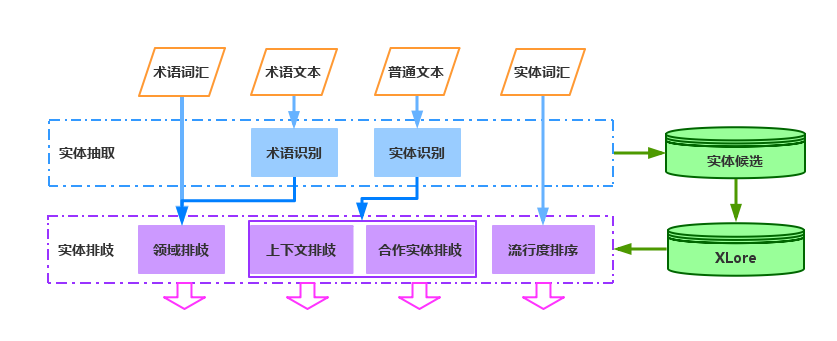
\includegraphics[width=1\columnwidth]{entity-linking-architecture}
  \caption{XLore 实体链接接口框架图}
  \label{fig:entity-linking-architecture}
\end{figure}

\subsection{实体抽取}
对于给定的长文本,我们引入成熟的实体或术语抽取工具提取出其中可以分析的实体文本,包括:
\begin{itemize}
\item 通用领域实体抽取,中文使用开源中文分词工具jieba\footnote{\url{https://github.com/fxsjy/jieba}},获得其中人名(nr)、地名(ns 和nsf)、机构团体名(nt)和其他专有名词(nz)作为待链接实体;英文使用斯坦福文本解析工具\footnote{\url{http://nlp.stanford.edu/software/lex-parser.shtml}}获取人物(PERSON)、地点(LOCATION)和组织机构(ORGANIZATION)三类实体。
\item 学术领域实体抽取使用来自微软的学术术语抽取工具。
\end{itemize}

\subsection{实体候选生成}

实体候选从名称-实体词典中,通过名称获取相应的所有实体。其中,中英文名称-实体词典从中英文维基百科、百度百科、互动百科中抽取,选取以下几种元素构成:

\begin{enumerate}[1.]
\item 各百科的词条标题:百科中的每个词条都描述唯一实体,并维护着这个实体的相关信息。一般来说,词条标题是该实体公认的、最普遍的名称。对于无歧义的标题,记录其完整标题即可。然而,有些标题有多种含义。在百科中,如果一个标题有歧义,百科会通过在标题后加入分类信息来实现消歧,比如百度百科中,苹果(蔷薇科苹果属果实)代表一种水果,苹果(苹果产品公司)代表美国一家高科技公司,这种情况,标题“苹果”为实体“苹果(蔷薇科苹果属果实)”的一个名称。
\item 各百科的文本内链接:百科词条的文本中,经常会有一些实体名称,以超链接的形式存在,指向该实体对应的词条。这个超链接的锚文本,可以看作是指向实体的同义词或别称。
\item 各百科的消歧页面:如果一个名称可能对应多个实体,百科会为其创建一个歧义页面,供用户按所需选择词条。比如,“苹果”是一个歧义词汇,则歧义页面中会列举“苹果(蔷薇科苹果属果实)”、“苹果产品公司”等词条。维基百科通过“苹果\_(消歧义)”这样的页面\footnote{https://zh.wikipedia.org/wiki/苹果\_(消歧义)}
展示词条,百度百科则通过为“苹果”父词条\footnote{\url{http://baike.baidu.com/view/1331.htm?force=1}}创建subview子词条来进行区分,如果一个词条没有歧义,则它的网页地址以id定位;如果一个词条有多种意思,则它的id页面为歧义页面,各子词条网址用subview id定位。消歧页面对于抽取实体的别称也有很大贡献。
\item 维基百科的重定向页面: 维基百科通过不断进行词条整理与更新,对一些陈旧的、非标准词条,或公认的缩写名称、别称等,将其自动定位到同一实体的标准词条页面上。原来的旧名称、缩写等可以看作实体的名称。比如中文维基中,“Microsoft”会被重定向到“微软”页面。
\end{enumerate}

以2016年3月的中英文维基百科、2014年12月的百度百科、互动百科为数据源,我们获得名称-实体关系数量如表\ref{tab:mention-entity}所示:

\begin{table}[htb]
  \centering
  \caption{名称-实体关系对抽取数量统计}
  \label{tab:mention-entity}
    \begin{tabular}{lcccc}
      \toprule[1.5pt]
      {\heiti 类型} & {\heiti 英文维基} & {\heiti 中文维基} & {\heiti 百度百科} & {\heiti 互动百科} \\\midrule[1pt]
      标题       & 16.345,549 & 2,739,609 & 5,794,412 & 5,590,173 \\
      内链接     & 45,650,452 & 6,784,030 & 5,875,459 & - \\
      消歧页面   & 240,578    & 2,550     & 174,862 & 24,158 \\
      重定向页面 & 2,759,377  & 362,767   & -  & - \\
      合并总对数 & 55,834,865 & 8,607,098 & 7,640,773 & 5,590,173 \\
      \bottomrule[1.5pt]
    \end{tabular}
\end{table}

抽取结果合并后,获得中英文名称-实体对应关系总数量为67,429,935对。我们只保留在XLore中能命中的实体,最终获得{\heiti 23,635,510}对关系。平均每个实体有1.97个名称,每个名称可能对应1.32个实体。
%17845907个mention, 11987986个entity

在抽取过程中,我们对名称-实体的出现频数进行了记录,用于之后的排歧工作。以\textit{名称 \ 实体知识库uri \ 出现频数}为格式存储数据,并以名称为索引,将数据导入到MySQL数据库中,便于查询。

\subsection{实体消歧方法}
实体消歧主要是对候选实体的匹配可能性进行排序,
对于通用领域的名称查询,因为没有任何上下文信息,我们只能直接以流行度(出现频数)从高到低排序,返回受到广泛认可的一个或多个实体信息。
对于学术领域的查询,我们利用知识库特有的分类体系,凭借领域约束,将实体的查找限制在相关概念下。

对于通用领域的文本查询,我们根据上下文,为每个名称返回最相关的实体。具体来说,对于给定名称,为其每个候选实体计算背景相关度,最相关的最可能为所求实体。
给定一段文本$T$,经过实体抽取后获得实体名称集合$M$,对于$m_i \in M$,计算$m_i$的实体候选$c_{i,j} \in C(m_i)$的相关度:
\begin{itemize}
\item 1.  计算上下文相关度($R_a$):认为自身信息与上下文有关的实体更相关,提取名称文本$T$,与实体的摘要$A(c_{i,j})$进行余弦相似度计算。

\item 2.  计算合作实体相关度($R_e$):认为与文中其他实体有语义关系的实体更相关,提取根据文中其他名称$M'=$对应的实体候选$C(M') = $,与本名称的实体候选的相关实体,即文本中的链接实体$I(c_{i,j})$做交集。
\begin{equation}
{ R }_{ e }=\frac { \left| C\left( M' \right) \cap I\left( { c }_{ i,j } \right)  \right|  }{ \left| I\left( { c }_{ i,j } \right)  \right| +1 }
\end{equation}

\item 3.  取两个相关度的最大值。
\begin{equation}
R = \max{ \left(R_a, R_e \right)}
\end{equation}
\end{itemize}
$R_{i,j}$ 即为实体候选$c_{i,j}$与名称$m_i$的相关度,$R_{i,j}$越大,$c_{i,j}$越可能是所求实体。

\subsection{实体链接接口的应用}
实体链接接口的学术领域名称查找功能,应用在Aminer学术搜索系统\footnote{\url{https://aminer.org/}}的学术知识展示模块上,如图\ref{fig:el-aminer}所示:用户在搜索学术领域词汇时,右边会显示该词汇对应的学术实体信息及其相关上下文概念。
\begin{figure}[ht]
  \centering
  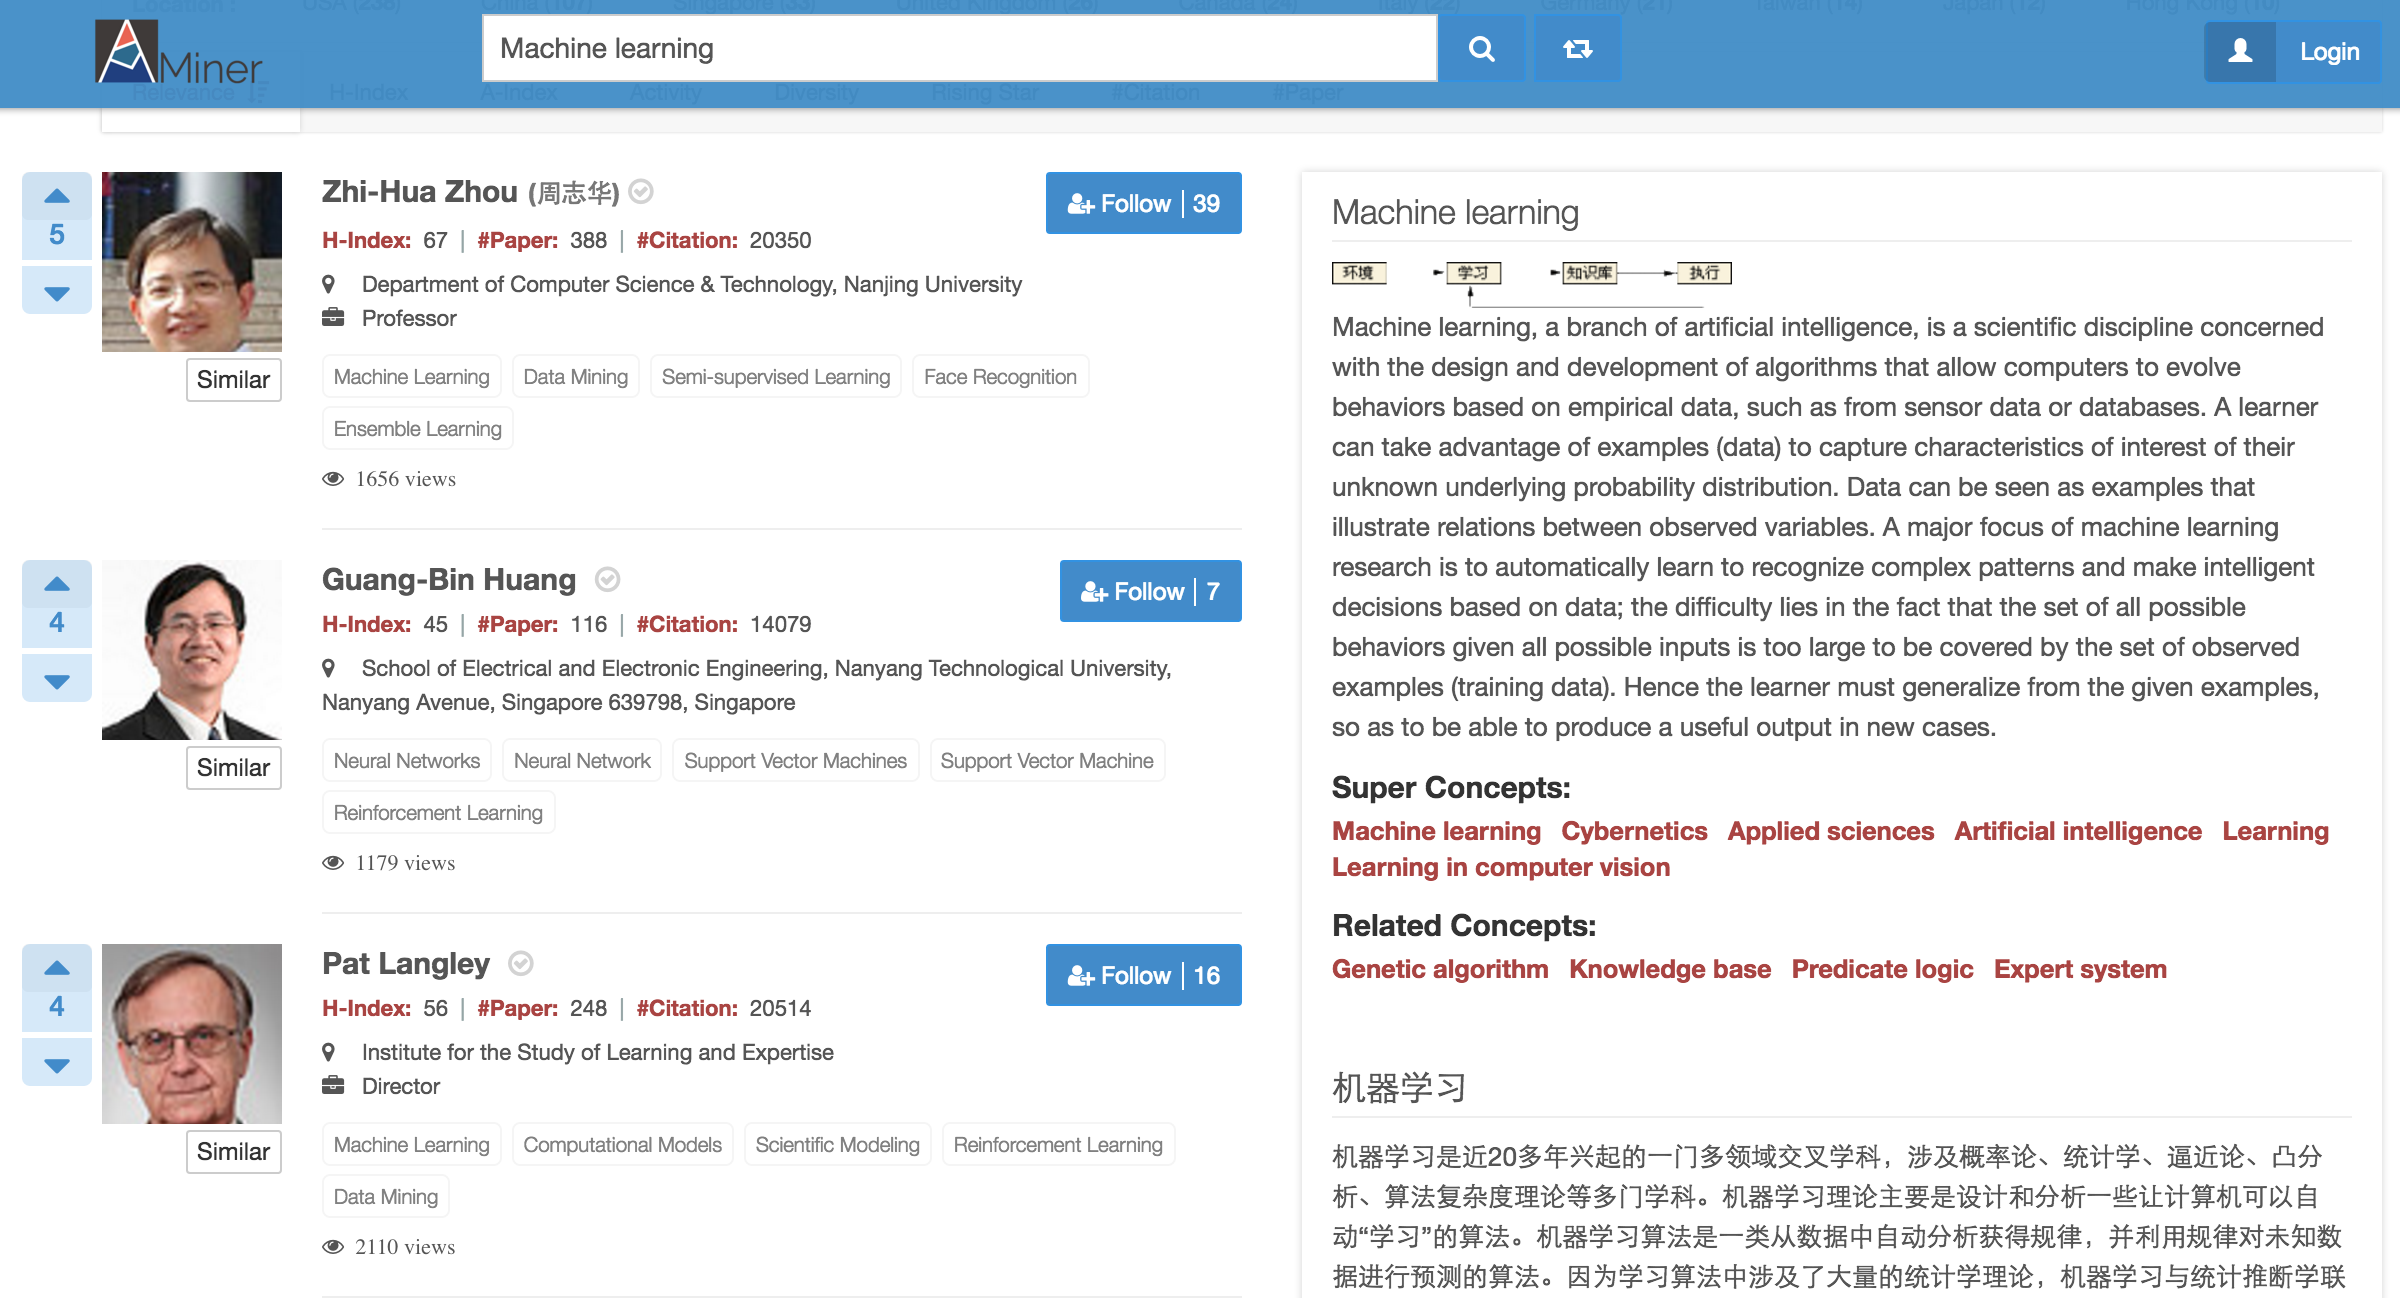
\includegraphics[width=0.8\columnwidth]{el-aminer}
  \caption{XLore实体链接接口在Aminer上的应用}
  \label{fig:el-aminer}
\end{figure}

通用领域名称查找功能,应用在新闻分析系统NewsMiner\footnote{\url{http://newsminer.net}}上,用于为新闻文本分析提供实体信息,如图\ref{fig:el-newsminer}所示。
\begin{figure}[ht]
  \centering
  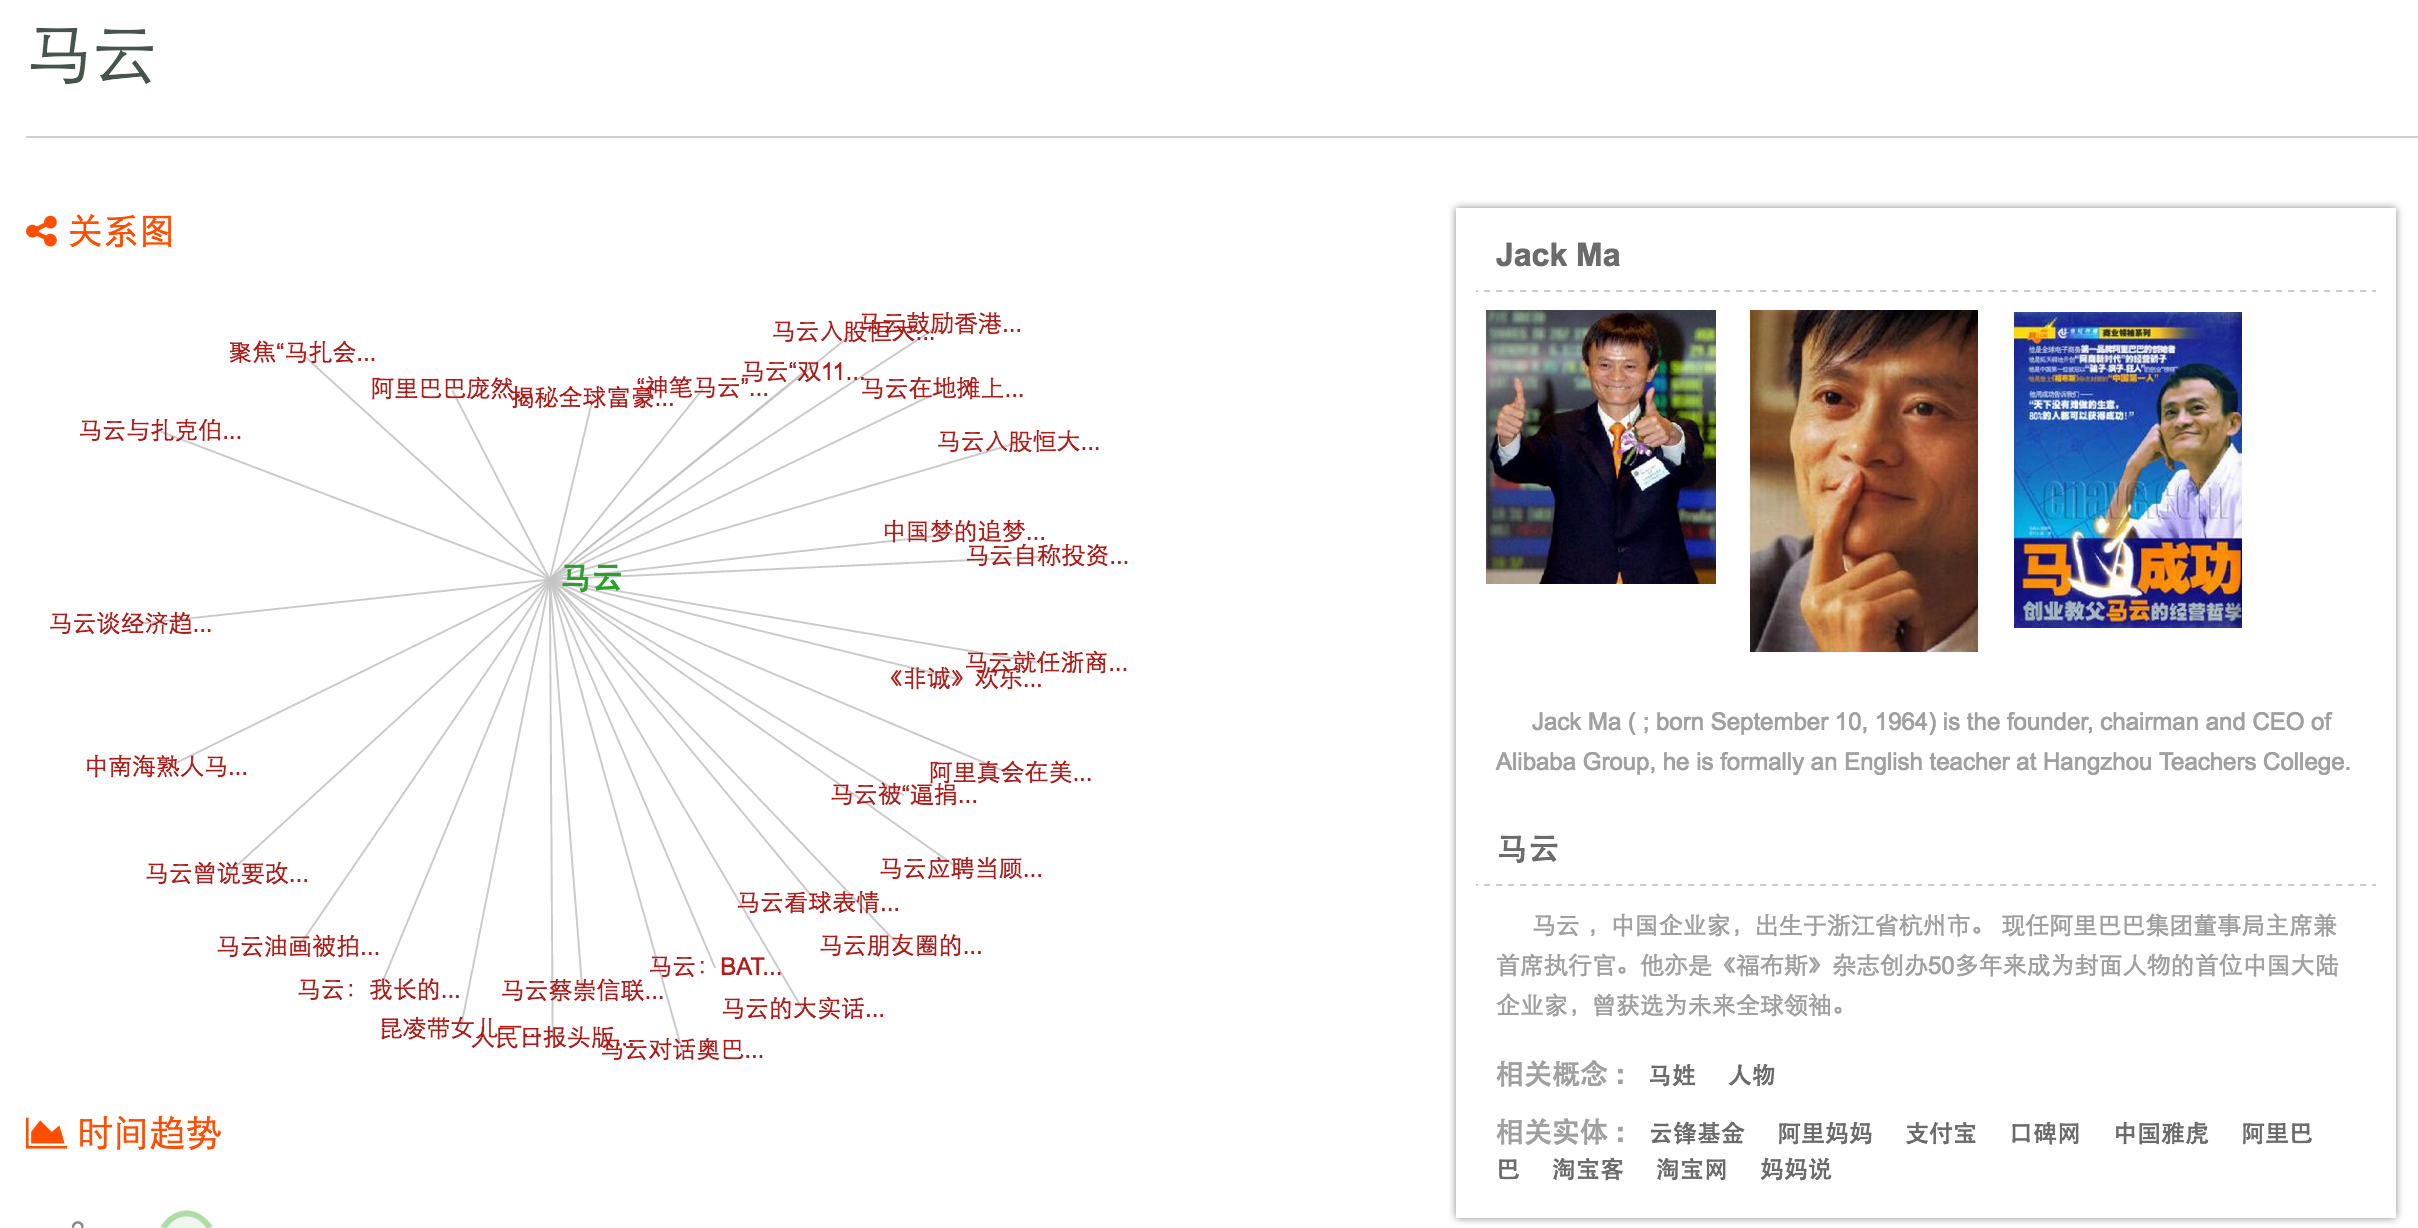
\includegraphics[width=0.8\columnwidth]{el-newsminer}
  \caption{XLore实体链接接口在NewsMiner上的应用}
  \label{fig:el-newsminer}
\end{figure}

\section{本章小结}
本章主要介绍融合多个在线百科数据,构建跨语言知识库的方法。我们从网页中抽取结构化数据并统一数据格式,生成并扩展跨语言链接信息来融合双语知识,最终获得的跨语言知识库XLore共包含663,740个概念,56,449个属性以及10,856,042个实例。

接下来,我们对XLore系统进行了详细介绍。为了进一步了解数据情况,搭建了XLore网站,通过搜索、可视化等功能将数据直观地展现出来。同时,为了提高知识库的可用性,开发了实体链接接口,提供通用领域与指定领域的语义信息,也为下一步更精确的实体链接工作做好铺垫。

